
\item[\ding{226}] \textbf{Paramètres pour la stratégie combiné de l'Oscillateur Stochastique et de la moyenne mobile convergence Divergence.}

\begin{itemize}
    \item[$\rightarrow$] Différence entre périodes.
    \par{
    Comme vu précédemment dans le cas de la stratégie des Moyennes Mobiles, nous allons choisir 
    une période pour la moyenne mobile exponentielle lente qui fait au moins le double de la 
    période de la moyenne mobile rapide.
    En plus des Moyennes Mobiles exponentielles rapide et lente, nous avons également testé des 
    périodes pour la fourchette de temps dans le cas de l'Oscillateur Stochastique, ainsi que 
    différentes périodes pour la ligne de signal qui représente la moyenne mobile arithmétique de la 
    MACD.
    Au total, nous avons obtenu \textbf{142560} combinaisons possibles ; soit allant de 20 à 59 pour la 
    période de la moyenne mobile exponentielle rapide, de 40 à 159 pour la période de la moyenne 
    mobile lente, de 3 à 6 pour le signal, et de 10 à 20 pour la fourchette de période de 
    l'Oscillateur Stochastique. }


    \item[$\rightarrow$] Taux de réussite des transactions.
    Dans cette partie, nous allons choisir les combinaisons de périodes ayant au moins fait un bénéfice 
    de \textbf{80\%}.
    Après ce filtrage, nous pouvons observer qu'il y a un nombre total de \textbf{120087} de combinaisons
    de périodes qui respectent cette condition dans le cas de l'application de la stratégie sur l'indice 
    BRVM-Agriculture et un total de \textbf{137935} pour l'indice BRVM-Services-Publics.  
    

    \item[$\rightarrow$] Taux de bénéfice.
    Parmi les 120087 observations restantes, nous remarquons que 1778 donnent un maximum de bénéfice 
    de 14,5\% et ont généré une seule transaction effectuée. Cela est dû au fait que le cours de l'actif 
    est monté durant toute la période allant de juillet 2020 à mai 2022, et que la moyenne mobile exponentielle 
    accorde une grande pondération aux données récentes. 
    De plus, nous avons observé deux combinaisons de périodes qui ont fait un 
    maximum de bénéfice de 37,366\%.
    Nous reprenons donc les simulations, mais cette fois-ci sur des périodes allant
    de 10 à 55 pour la période de la moyenne mobile exponentielle rapide, et de 
    25 à 100 pour la période de la moyenne mobile exponentielle lente,
    de 4 à 6 pour la ligne de signal, et de 14 à 20 pour la fourchette de période de
    l'Oscillateur Stochastique. 
    Au total, nous obtenons \textbf{56196} nouvelles observations.
    Après analyse, il ressort qu'une combinaison de périodes génère un maximum de bénéfice
    de 29,105\% pour l'indice BRVM-Agriculture, et deux différentes combinaisons de 
    périodes ont fait un bénéfice de 39,758\% soit (24,37) et (25,36).
    

\item[$\rightarrow$] Robustesste.
    \begin{center}
        \textbf{"BRVM-agri" }
    \end{center}
    \begin{table}[ht]
        %\rowcolors{2}{myblue}{white}
        \centering
        \caption{Période voisins du couple (25,10) pour la BRVM-Agriculture}
        \begin{tabular}{p{1.5cm}p{1.5cm}p{1.5cm}p{1.5cm}p{1.5cm}p{1.5cm}p{1.5cm}}
            \hline
            Longue & Courte & Bénefice & Positive &Négative &Niveau &Signal\\
            \hline
            24	&9	&29.09	&5	&1	&20	&4	\\  
            25	&9	&25.515	&5	&1	&20	&4	\\  
            26	&9	&29.105	&5	&1	&20	&4	\\  
            24	&10	&25.515	&5	&1	&20	&4	\\  \hline
            \cellcolor{myblue}25	&\cellcolor{myblue}10	&\cellcolor{myblue}29.105	
            &\cellcolor{myblue}5	&\cellcolor{myblue}1	&\cellcolor{myblue}20	&\cellcolor{myblue}4 \\ \hline  
            26	&10	&18.682	&4	&1	&20	&4	\\  
            24	&11	&18.682	&4	&1	&20	&4	\\  
            25	&11	&20.111	&4	&1	&20	&4	\\  
            26	&11	&18.256	&4	&1	&20	&4	\\ 
            \hline
        \end{tabular}
    \end{table}%

    \par{D'après l'analyse du tableau ci-dessus, nous pouvons remarquer qu'une légère modification de la 
    période de la moyenne mobile exponentielle lente et rapide ne modifie pas largement le taux de 
    bénéfice. En effet, pour une modification de la période de la moyenne mobile exponentielle rapide 
    et lente respectivement de 24 à 26 et de 9 à 11, nous pouvons observer une variation de bénéfice
    entre 18,256\% et 29,105\%. Dans le même temps, nous remarquons pour les observations voisines une transaction 
    négative qui survient sur un total de 5 transactions pour les périodes (26,10), (25,11), (24,11) et 
    (26,11), et pour un total de 6 transactions pour les périodes (24,9), (26,9), (26,9) et (24,10). 
    Nous pouvons déduire que les résultats restent moyennement stables pour les périodes (25,10). Nous en 
    déduisons que les périodes 25 pour la moyenne mobile exponentielle lente, 10 pour la moyenne 
    mobile exponentielle rapide, 20 pour la fourchette de temps de l'Oscillateur Stochastique et 
    4 pour la ligne de signal sont robustes dans l'application de la stratégie combinée de l'Oscillateur Stochastique et 
    de la Moyenne Mobile Convergence Divergence sur l'indice BRVM-Agriculture.}
    
  
    \begin{center}
        \textbf{"BRVM-Services-Publique" }
    \end{center}
    \begin{table}[ht]
        %\rowcolors{2}{myblue}{white}
        \centering
        \caption{Période voisins du couple (25,36) pour la BRVM-Services-Publics}
        \begin{tabular}{p{1.5cm}p{1.5cm}p{1.5cm}p{1.5cm}p{1.5cm}p{1.5cm}p{1.5cm}}
            \hline
            Longue & Courte & Bénefice & Positive &Négative &Niveau &Signal\\
            \hline
            35	&24	&26.048	&5	&0	&19	&6	\\ 
            36	&24	&27.304	&5	&0	&19	&6	\\ 
            37	&24	&39.758	&5	&0	&19	&6	\\ 
            35	&25	&27.304	&5	&0	&19	&6	\\ \hline
            \cellcolor{myblue}36	&\cellcolor{myblue}25	&\cellcolor{myblue}39.758	
            &\cellcolor{myblue}5	&\cellcolor{myblue}0	&\cellcolor{myblue}19	&\cellcolor{myblue}6	\\ \hline
            37	&25	&38.151	&5	&0	&19	&6	\\ 
            36	&26	&38.151	&5	&0	&19	&6	\\ 
            37	&26	&38.151	&5	&0	&19	&6	\\ 
            \hline
        \end{tabular}
    \end{table}%
    \par{D'après l'analyse du tableau ci-dessus, il ressort qu'une variation de la période lente entre 
    35 et 37 et une variation de la période rapide entre 24 et 26 font varier le pourcentage de 
    bénéfice de 26,048\% à 38,151\%. Notons également que pour les périodes 
    (37,25), (36,26) et (37,26), le bénéfice reste stable et ne change pas. De plus, pour toutes 
    les périodes avoisinant le couple (25,36), le nombre de transactions reste le même avec 100\% de 
    transactions positives. Nous en déduisons alors que les périodes 25, 36, 19 et 6, respectivement 
    pour la moyenne mobile rapide, lente, la fourchette de période de l'Oscillateur 
    Stochastique et la période de la ligne Signal, sont robustes dans le cas de l'application de la stratégie
    combinée de l'Oscillateur Stochastique et de la Moyenne Mobile Convergence Divergence
    sur l'indice BRVM-Services-Publics.}
    
\end{itemize}
\end{itemize}
\textbf{Strategies de trading.}
\begin{itemize}
\item[\ding{226}] \textbf{Strategie des Moyennes Mobiles avec les périodes standard.} \\
\begin{center}     \textbf{"BRVM-Agriculture"-"BRVM-Services-Publics"}  \end{center}

\begin{figure}[h]
    \centering
    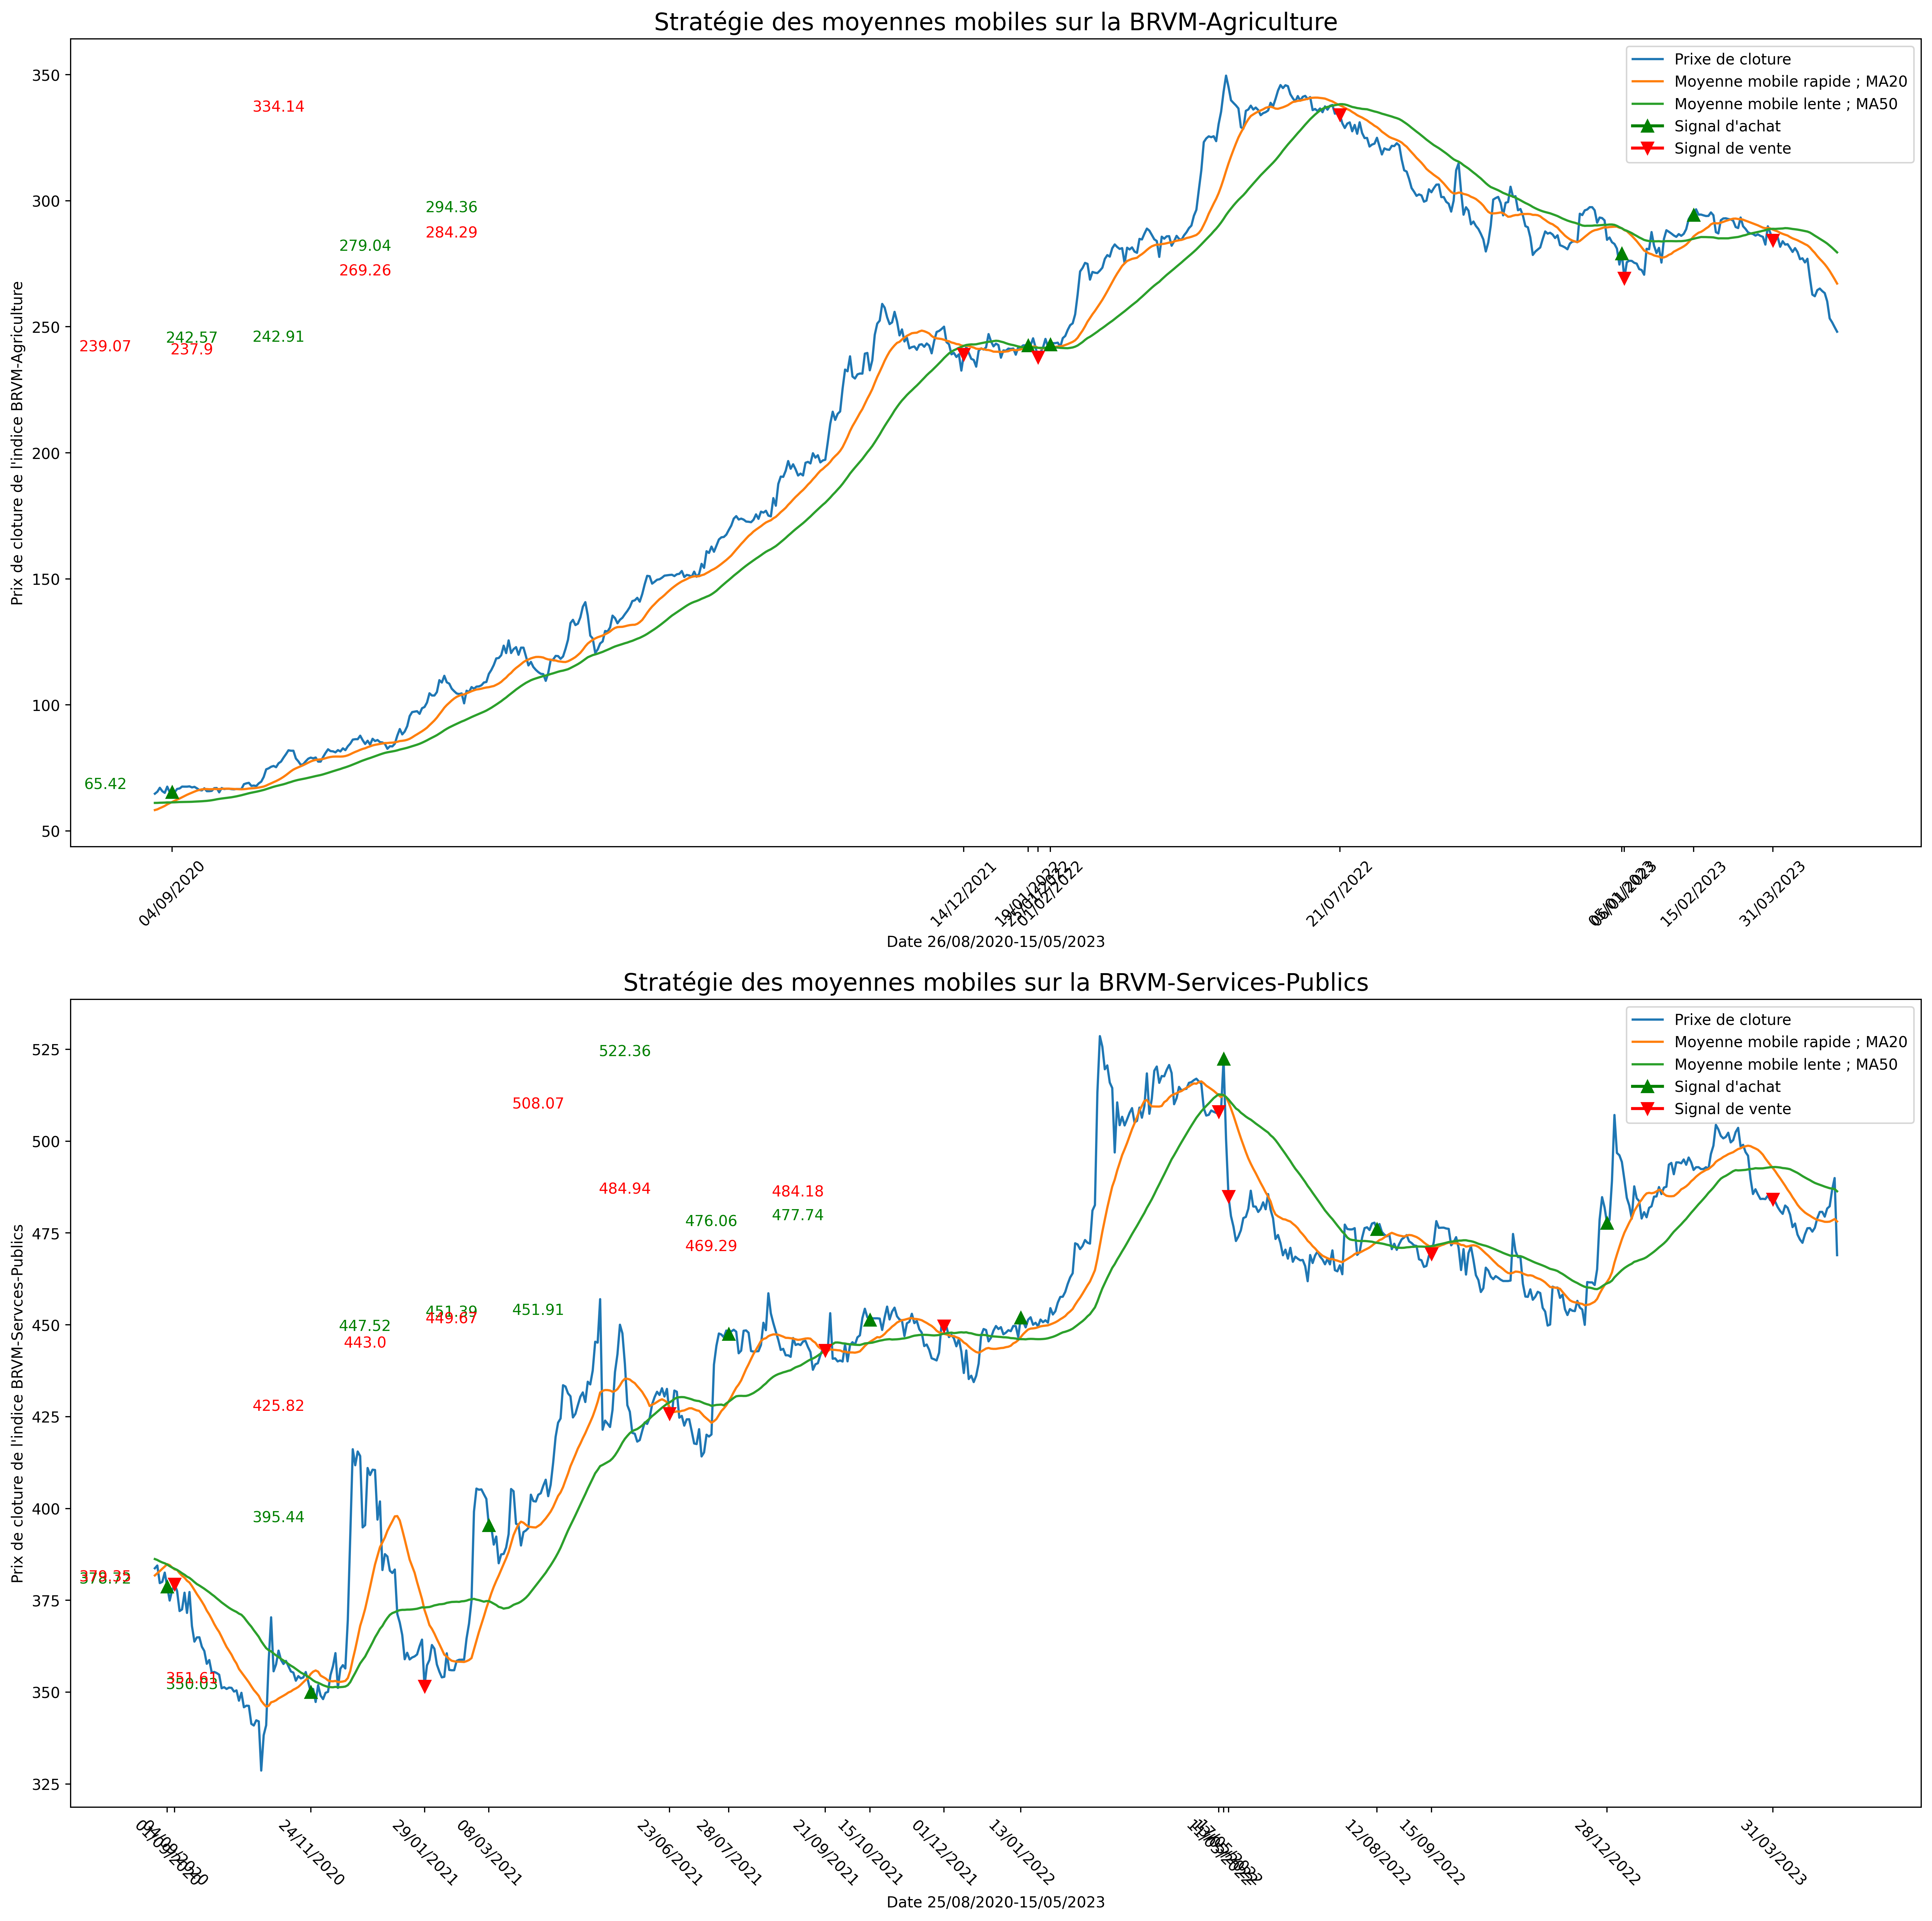
\includegraphics[width=1 \textwidth ]{img/MA-standard.png}
    \caption{Strategie des Moyennes Mobiles avec les périodes standard}
    \label{fig:Strategie des Moyennes Mobiles avec les périodes standard}
\end{figure}


\newpage

\item[\ding{226}] \textbf{Strategie Combine de MACD et de Stochastique avec les périodes standard.} \\
 \begin{center}     \textbf{"BRVM-Agriculture-BRVM-Services-Publics"}  \end{center}
\begin{samepage}
\begin{figure}[h]
    \centering
    \includegraphics[width=0.8 \textwidth ]{img/MACD-standard.png}
    \caption{Strategie Combine de MACD et de Stochastique avec les périodes standard}
    \label{fig:Strategie Combine de MACD et de Stochastique avec les périodes standard}
\end{figure}
\end{samepage}
\newpage

La figure 3.3 illustre la stratégie des Moyennes Mobiles sur les indices 
BRVM-Agriculture et BRVM-Services-Publics. L'analyse révèle que cette stratégie 
a généré 10 signaux d'achat et de vente sur l'indice BRVM-Agriculture, ainsi
qu'un total de 18 signaux d'achat et de vente sur l'indice BRVM-Services-Publics.
La première transaction réalisée sur l'indice BRVM-Agriculture a été la plus
 bénéfique, car le signal d'achat était de 65,42 Fcfa, tandis que le signal 
 de vente était de 239,07 Fcfa. Cependant, les deux dernières transactions 
 utilisant la stratégie des Moyennes Mobiles se sont soldées par des pertes.
  Ainsi, sur un total de 5 transactions, seules 2 ont été enregistrées, soit 
  un taux de réussite de 40%.
Concernant l'indice BRVM-Services-Publics, la stratégie des Moyennes Mobiles a
 généré un total de 18 signaux d'achat et de vente. Parmi ces 18 transactions 
 organisées, 14 ont été positives, représentant un taux de réussite de 77\%. 
 L'analyse des courbes révèle que la 6ème transaction a été la plus bénéfique, 
 avec un signal d'achat à un cours de 451,91 Fcfa et un signal de vente à un prix 
 de 508,07 Fcfa. De plus, entre le 11, 13 et le 17 mai 2022, on peut observer une 
 série de signaux d'achat et de vente causée par une chute, un pic, et une rechute 
 des cours entre les périodes allant du 10 mai 2022 (où l'indice valait 507,70 Fcfa)
  au 13 mai (où l'indice était à 522,36 Fcfa), pour finalement descendre à 
  500,63 Fcfa le lendemain.
En résumé, la stratégie des Moyennes Mobiles a généré un bénéfice total de 
\textbf{359,46\%} pour l'indice BRVM-Agriculture et un bénéfice total de 
\textbf{11,41\%} pour l'indice BRVM-Services-Publics."



La figure 3.4 illustre la stratégie combinée de l'Oscillateur Stochastique et de 
la moyenne mobile convergence divergence sur les indices BRVM-Agriculture et 
BRVM-Services-Publics. De son analyse, il ressort que la méthode combinée de 
l'Oscillateur Stochastique et de la MACD a donné un total de 3 signaux d'achat 
et de vente. 
Sur les trois signaux obtenus, une seule transaction a été réalisée, soit un signal
d'achat pour un cours de 311,58 Fcfa et un signal de vente à 294,52 Fcfa, ce qui
représente un faux signal et donc a donné lieu à une transaction négative. Par la
suite, un signal d'achat a été généré, mais malheureusement, dans la suite des 
données, il n'y a plus eu de signal de vente.
Au total, la stratégie combinée de l'Oscillateur Stochastique et de la moyenne 
mobile convergence divergence a donné un taux de bénéfice de \textbf{-5,48\%} sur 
la BRVM-Agriculture.
En ce qui concerne l'indice BRVM-Services-Publics, la stratégie a donné 9 signaux 
d'achat et de vente. Nous n'avons pas observé de fausses transactions, mais un signal
de vente très tôt à la 4ème transaction.
En somme, la stratégie a donné un bénéfice total de \textbf{29,79\%} sur l'indice 
BRVM-Services-Publics.


\newpage

\item[\ding{226}] \textbf{Strategie des Moyennes Mobiles (avec les nouveaux paramètres).}

\par{Maintenant que nous connaissons les périodes qu'il faut, nous allons appliquer la stratégie de 
trading basée sur la moyenne mobile sur les indices BRVM-Agriculture et sur les indices BRVM-Services-Publics.}

\begin{center}  \textbf{"BRVM-Agriculture"}  \end{center}
    \begin{figure}[h]
        \centering
        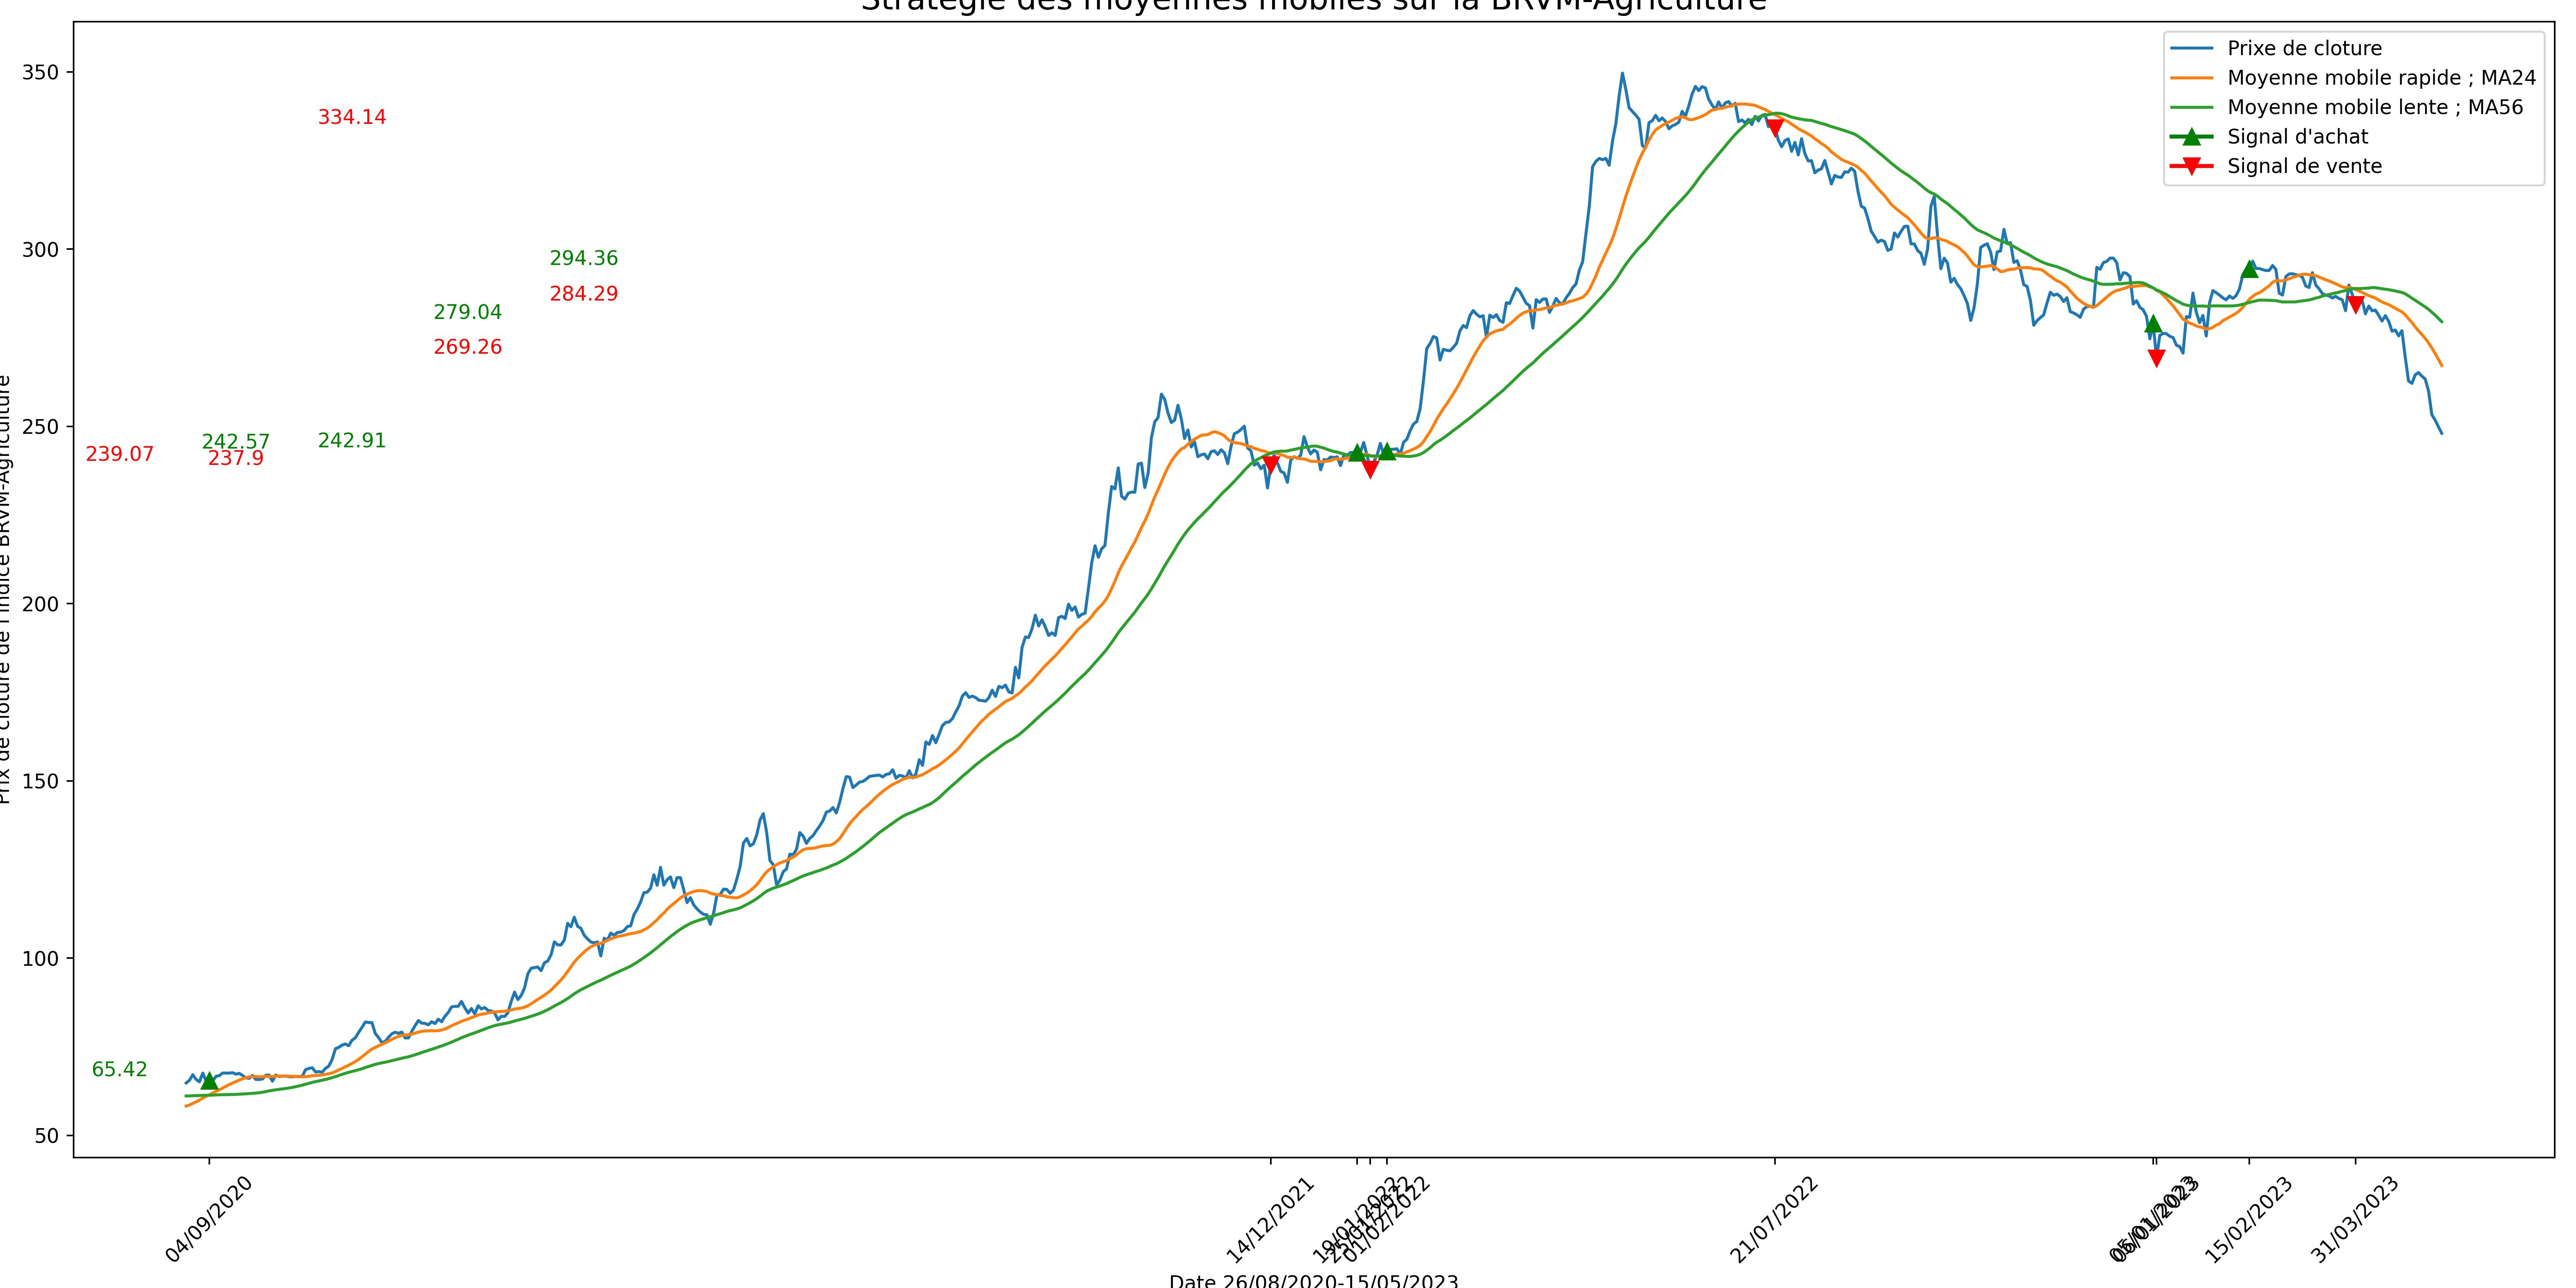
\includegraphics[width=1 \textwidth ]{img/MA-agri.jpg}
        \caption{Strategie des Moyennes Mobiles sur la BRVM-Agri}
        \label{fig:Strategie des Moyennes Mobiles sur la BRVM-Agri}
    \end{figure}
    \par{La figure ci-dessus illustre l'application de la stratégie des Moyennes Mobiles sur 
    l'indice BRVM-Agriculture. Cette représentation graphique présente les tendances de la 
    moyenne mobile arithmétique lente et de la moyenne mobile rapide, ainsi que les signaux 
    d'achat et de vente. L'analyse de cette figure révèle que la stratégie des Moyennes Mobiles 
    a généré un total de 8 signaux d'achat et de vente.

    Sur le graphique de gauche, nous pouvons observer des nombres en rouge et en vert. Le nombre 
    en vert représente le prix d'achat de l'actif après un signal d'achat, tandis que le nombre 
    en rouge représente le prix de vente au signal de vente. Ainsi, si le nombre en rouge est 
    inférieur au nombre en vert, cela signifie que la transaction a entraîné une perte.
    
    Dans la figure ci-dessous, nous pouvons remarquer que toutes les transactions sont positives,
     indiquant l'absence de faux signaux, ou presque. Toutefois, entre le 26 janvier 2022 et le 2 
     février 2022, nous avons observé deux signaux d'achat et de vente très rapprochés en raison 
     d'une fluctuation inhabituelle du cours de l'indice. Malgré cela, les transactions ont été un 
     succès car le prix d'achat était de 236,96 et le prix de vente de 242,91."
    La méthode des Moyennes Mobiles sur la BRVM-Agriculture à donner \textbf{367,167\%}}
    



    
    \begin{center}     \textbf{"BRVM-Services-Publics"}  \end{center}
    \begin{figure}[h]
        \centering
        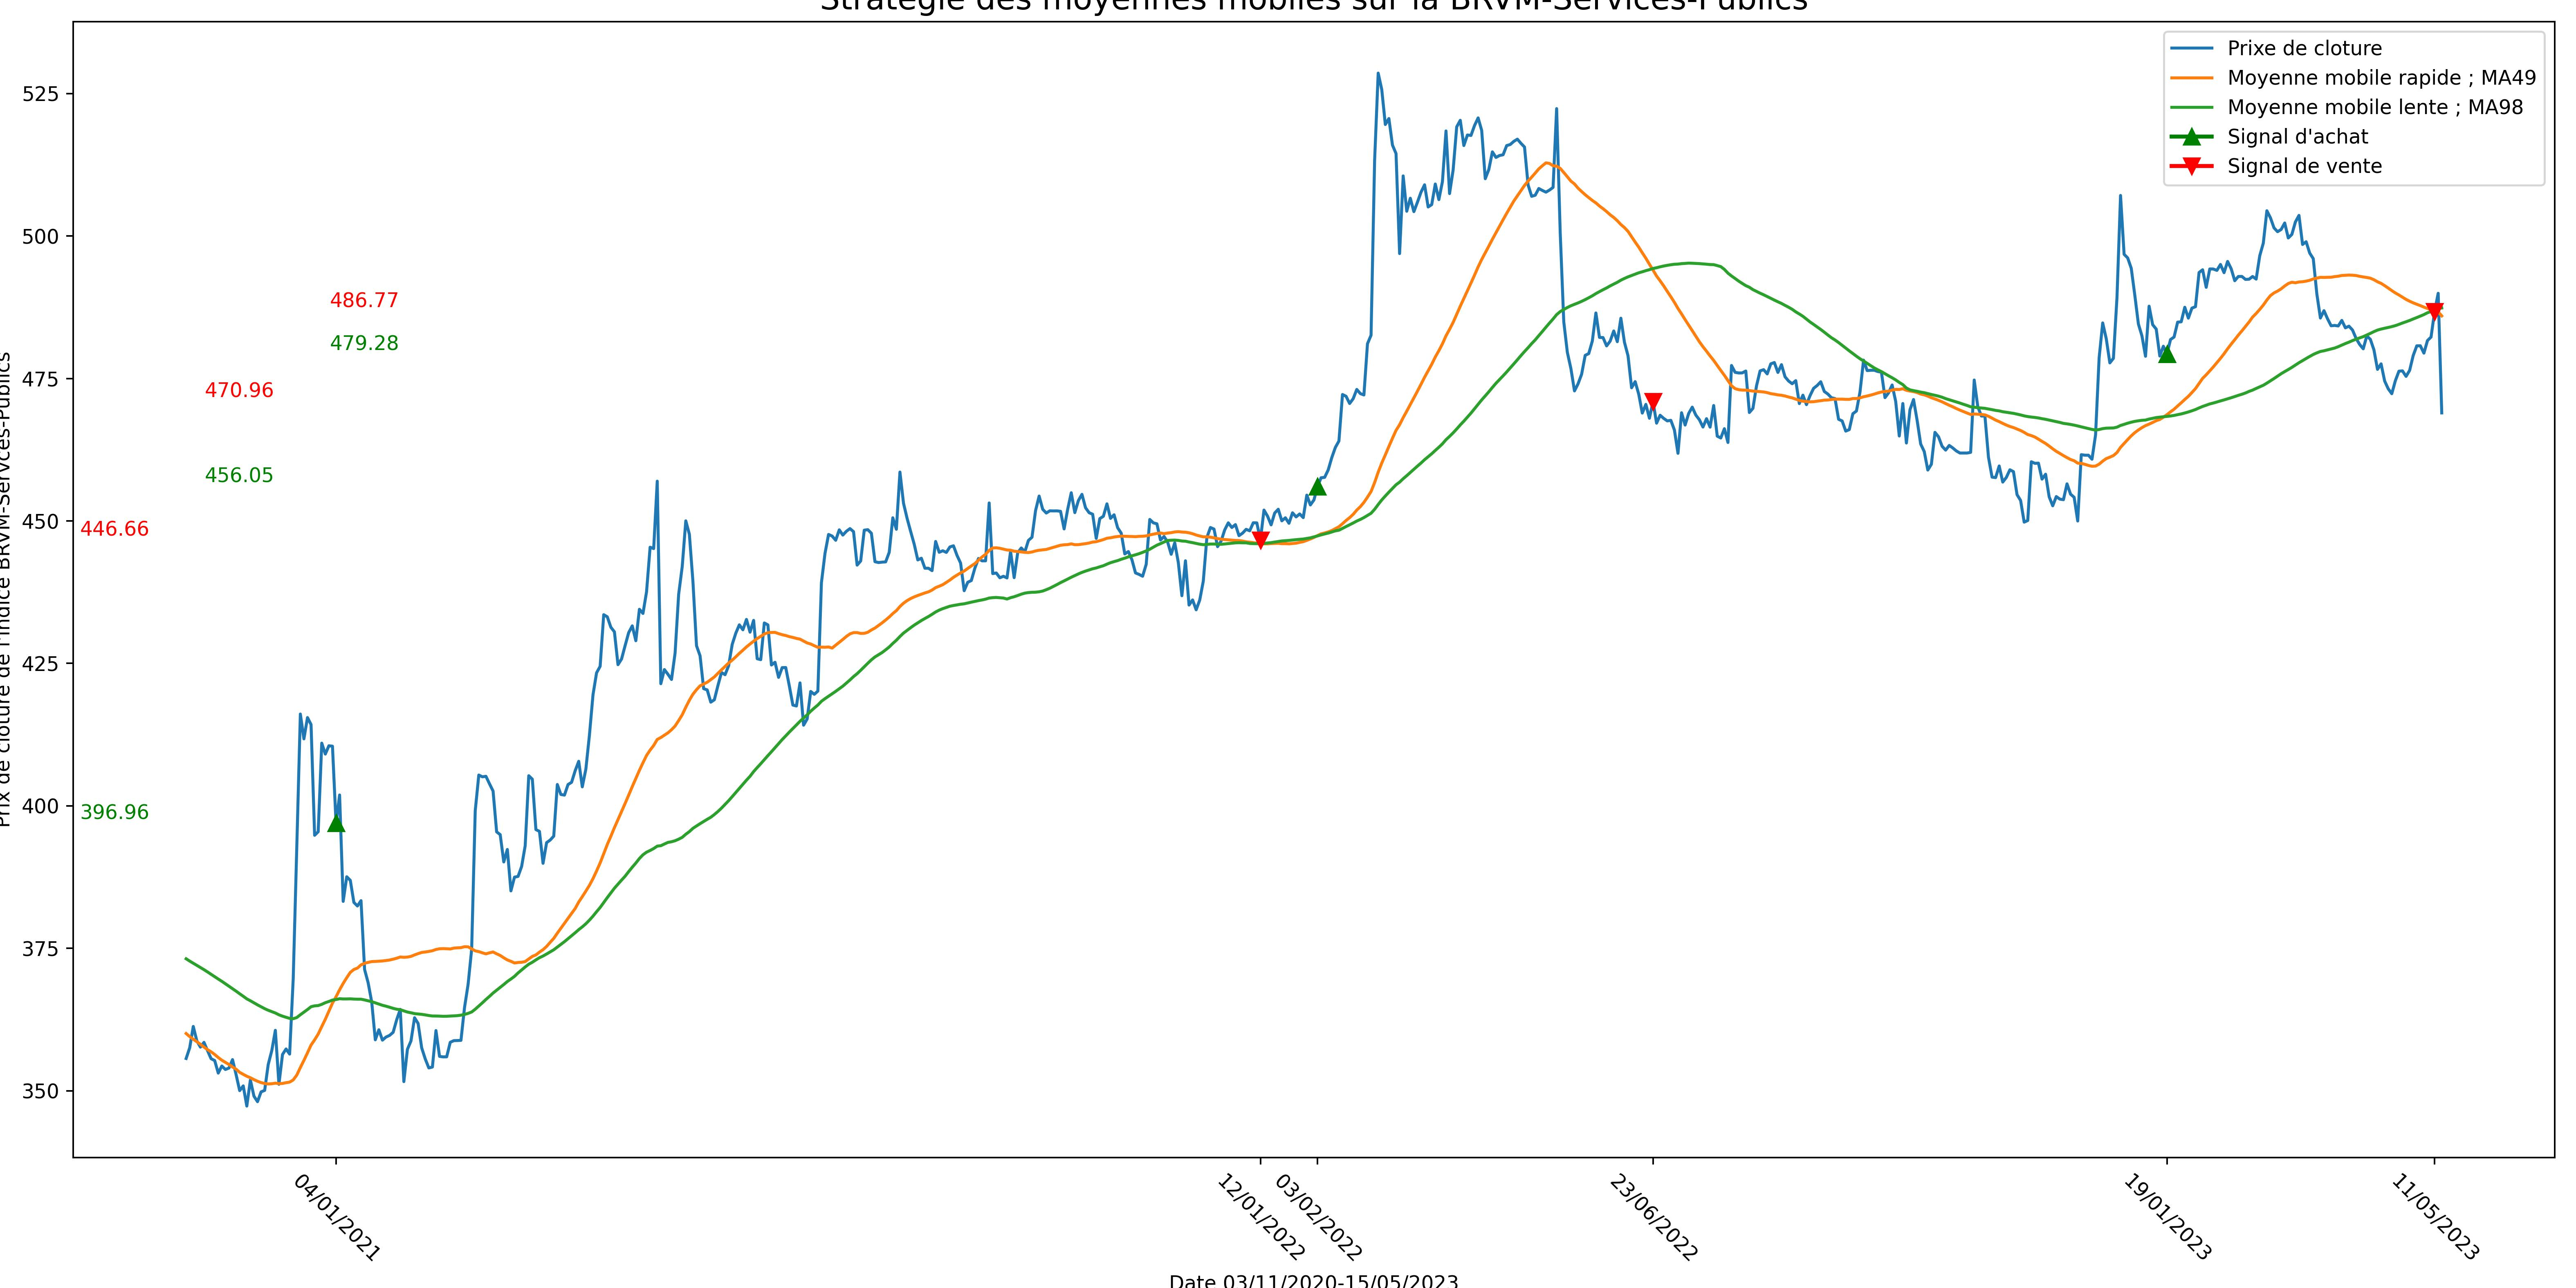
\includegraphics[width=1 \textwidth ]{img/MA-public.jpg}
        \caption{Strategie des Moyennes Mobiles sur la BRVM-Services-Publics}
        \label{fig:Strategie des Moyennes Mobiles sur la BRVM-Services-Publics}
    \end{figure}
    \par{
        La représentation graphique ci-dessus offre une vue de la stratégie de trading 
        des Moyennes Mobiles sur l'indice BRVM-Services-Publics. Dans le coin à droite ce trouve 
        des informations sur ce que représente chaque courbe. Ainsi nous pouvons lire que 
        la courbe en vert représente la moyenne mobile sur 98 jours ('lente') et celle orange la 
        moyenne mobile sur 48 jours ('rapide'). 
        De son analyse il ressort qu'un total de trois transactions on été effectuées dont la plus bénéfique 
        est la première transaction. En effet lors de cette transaction l'indice à été acheter au prix de 
        396,96 Fcfa et revendu à 446,66 Fcfa. 
        
        Remarquons cependant que le signal d'achat est un signal 
        légèrement en retard car il survient après un pique observer entre le 09 décembre 2020 et le 17 
        décembre 2020 ou le cours de l'indice est passe de 351,14 fcfa à 416,12 Fcfa. Il aurait été donc plus 
        bénéfique que le signal d'achat ait été générer un peux plus tôt. Mais cela est dur à ce mouvement 
        inhabituelle observer durant cette période de temps. 
        Le phénomène contraire s'observe également 
        au niveau de la deuxième transaction ou le signal de vente est venu un peu trop tardivement après un 
        que l'indice est atteint son plus grand pique.
        En somme la Stratégie des Moyennes Mobiles sur l'indice BRVM-Services-Publics à engendrer un bénéfice 
        total de \textbf{18,01 \%} }



\item[\ding{226}]\textbf{Strategie Combiné de l'Oscillateur Stochatique et de la 
Moyenne Mobile Convergence Divergence (avec les nouveaux paramètres).}

\begin{center}     \textbf{"BRVM-Agriculture"}  \end{center}
\begin{figure}[h]
    \centering
    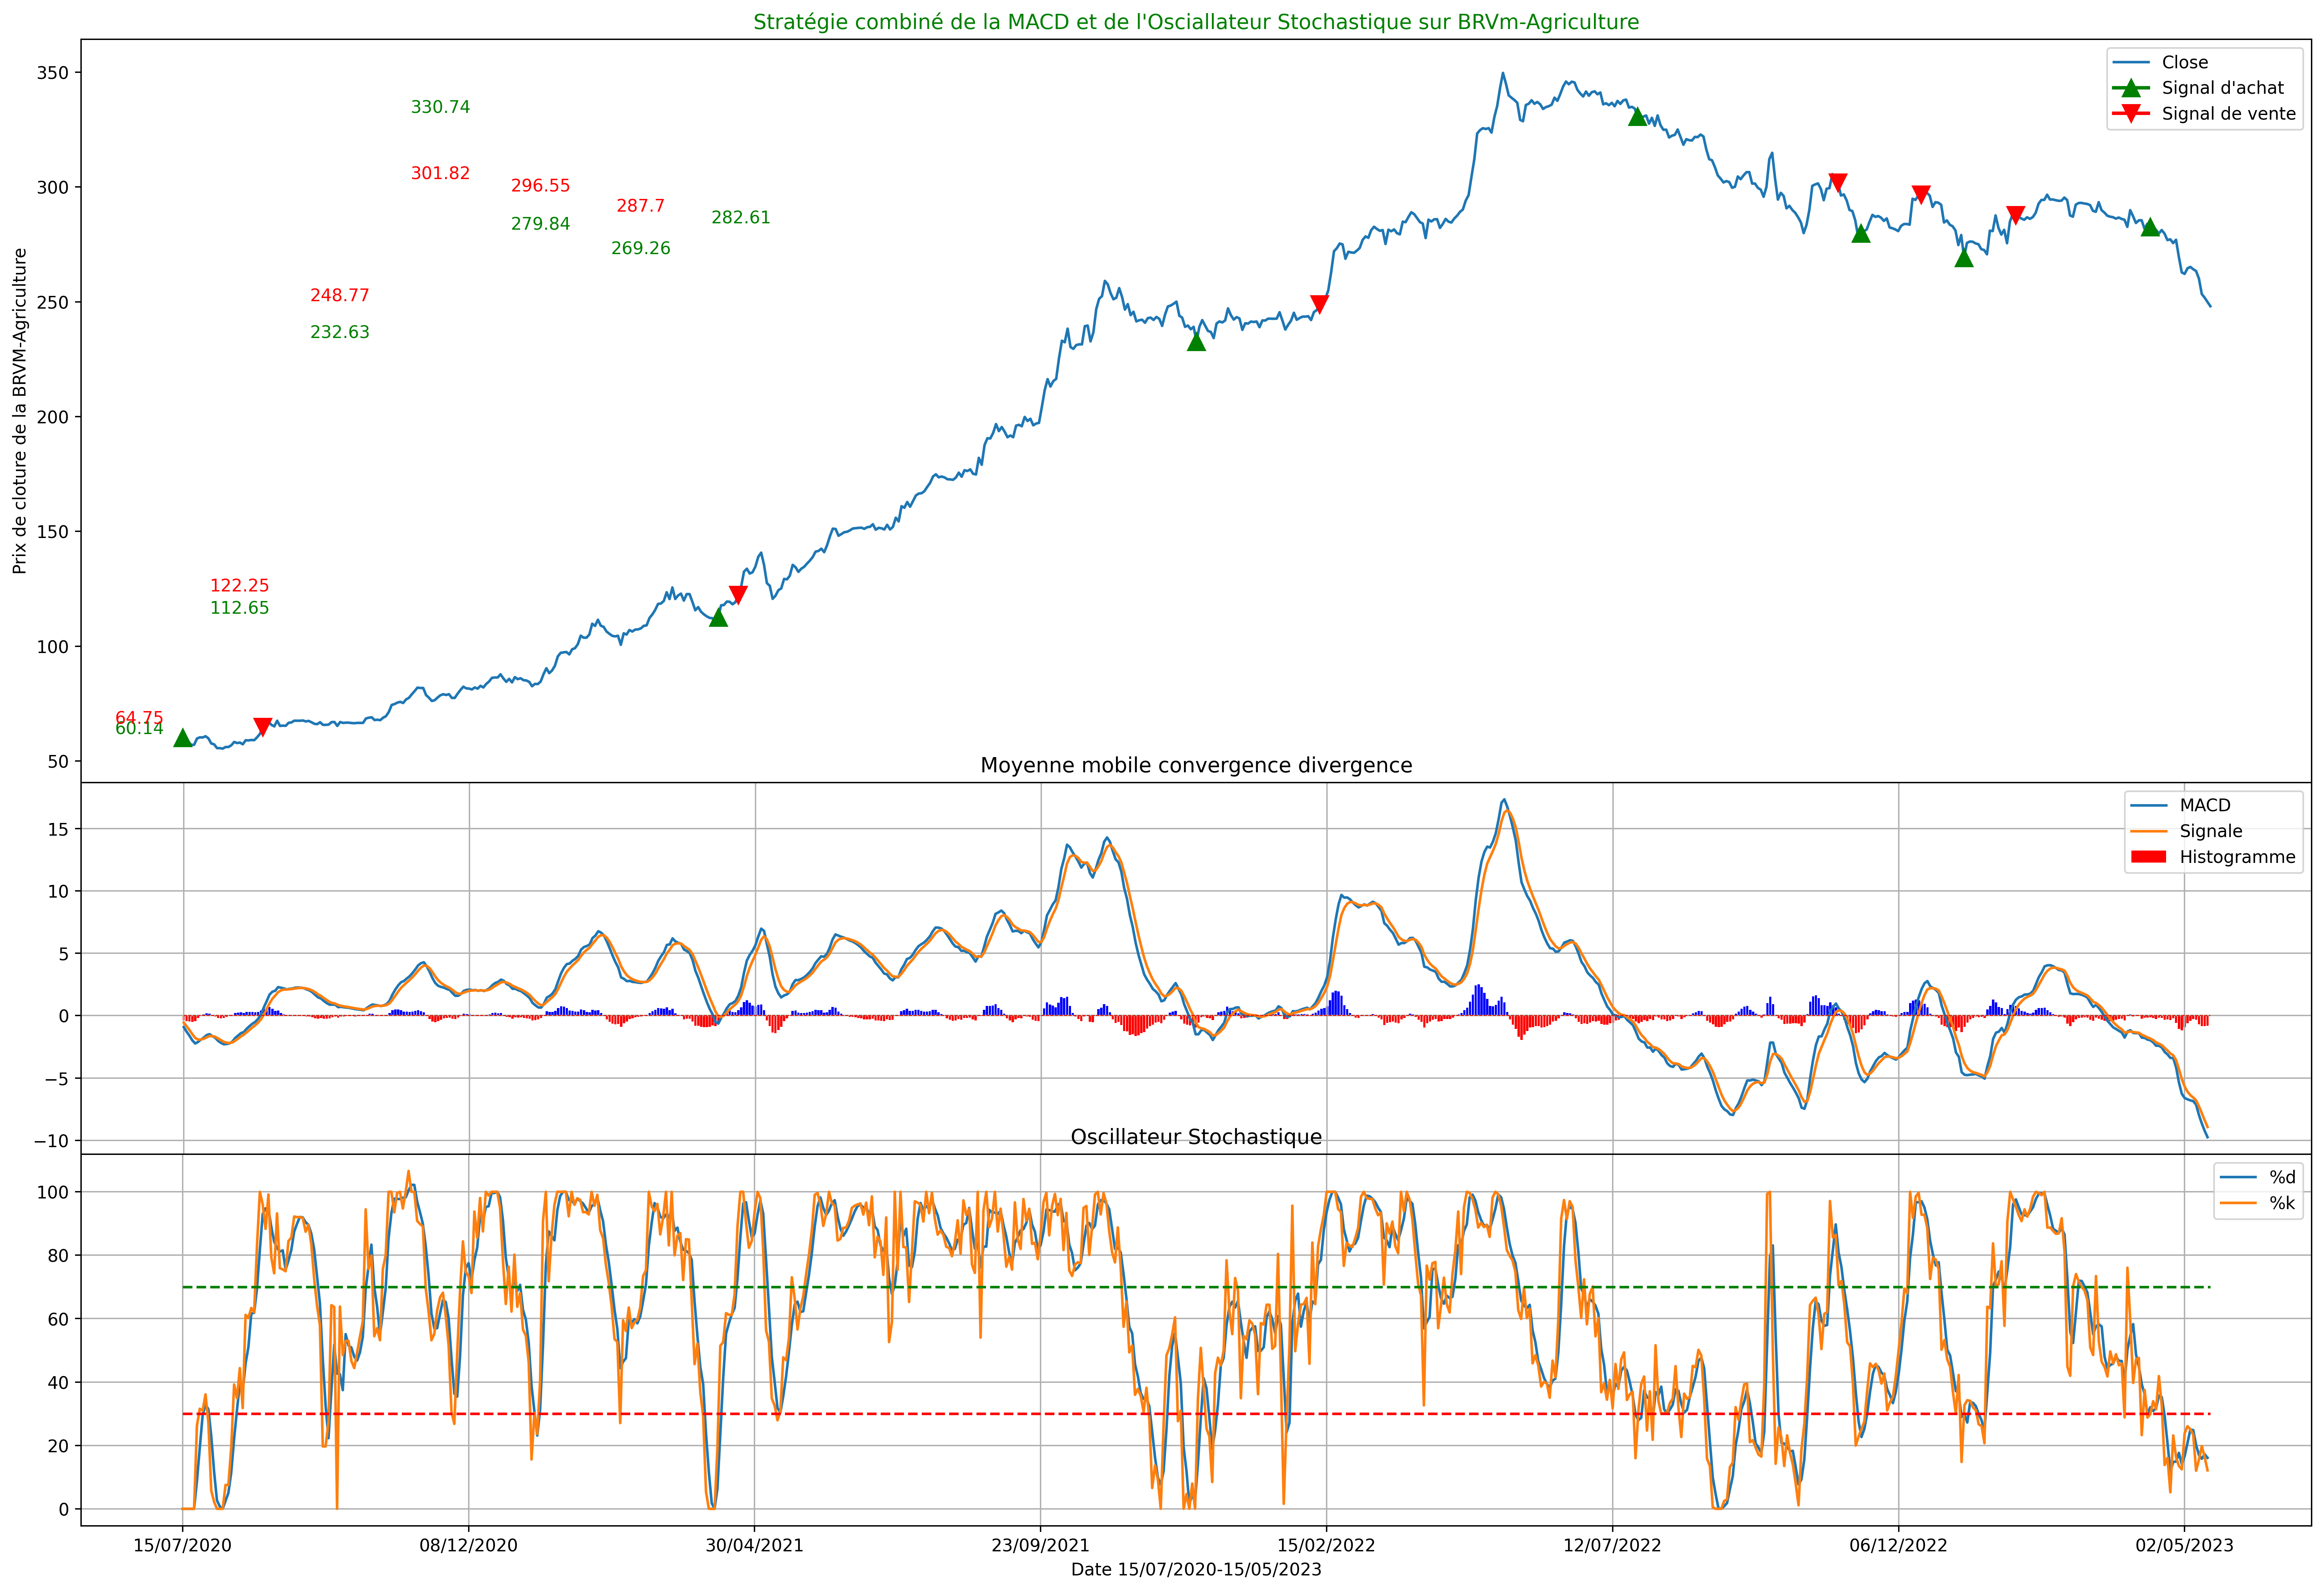
\includegraphics[width=1 \textwidth ]{img/MACD-Agri.png}
    \caption{Strategie Combine de MACD et de Stochastique sur l'indice Agriculture}
    \label{fig:Strategie Combine de MACD et de Stochastique sur l'indice Agriculture}
\end{figure}
\par{La représentation graphique ci-dessus, illustre la courbe du cours de l'indice BRVM-Agriculture , 
la Moyenne Mobile Convergence Divergence , ainsi que l'Oscillateur Stochastique. De cette
représentation graphique, nous pouvons observer que les courbes de l'Oscillateur Stochastique 
dépasse très fréquemment la barre des 70\% ce qui indique à chaque fois que le marché est dans 
un état de surachat ce qui représente un signal de vente. Cependant afin de valider 
ce signal il faut que la MACD soit supérieur à zéro. 
De plus on peut remarquer que 
après le 12 juillet 2022 une fluctuation inhabituelle des cours de l'indice, ce 
qui a générer un faux signal de vente et qui donc a conduit une perte au cours de cette
transaction. Suivant les cours des transactions en haut à gauche (du côté de la courbe des cours
de l'indice) nous pouvons observer que le prix d'achat de la valeur à cette transaction 
était de 330,74 Fcfa et son prix de vente de 301,81 Fcfa. 
Finalement la stratégie combinée
de l'Oscillateur Stochastique et de la Moyenne Mobile Convergence Divergence à donner un 
bénéfice total de \textbf{29,105\%} } 




\begin{center}     \textbf{"BRVM-Services-Publics"}  \end{center}
\begin{figure}[h]
    \centering
    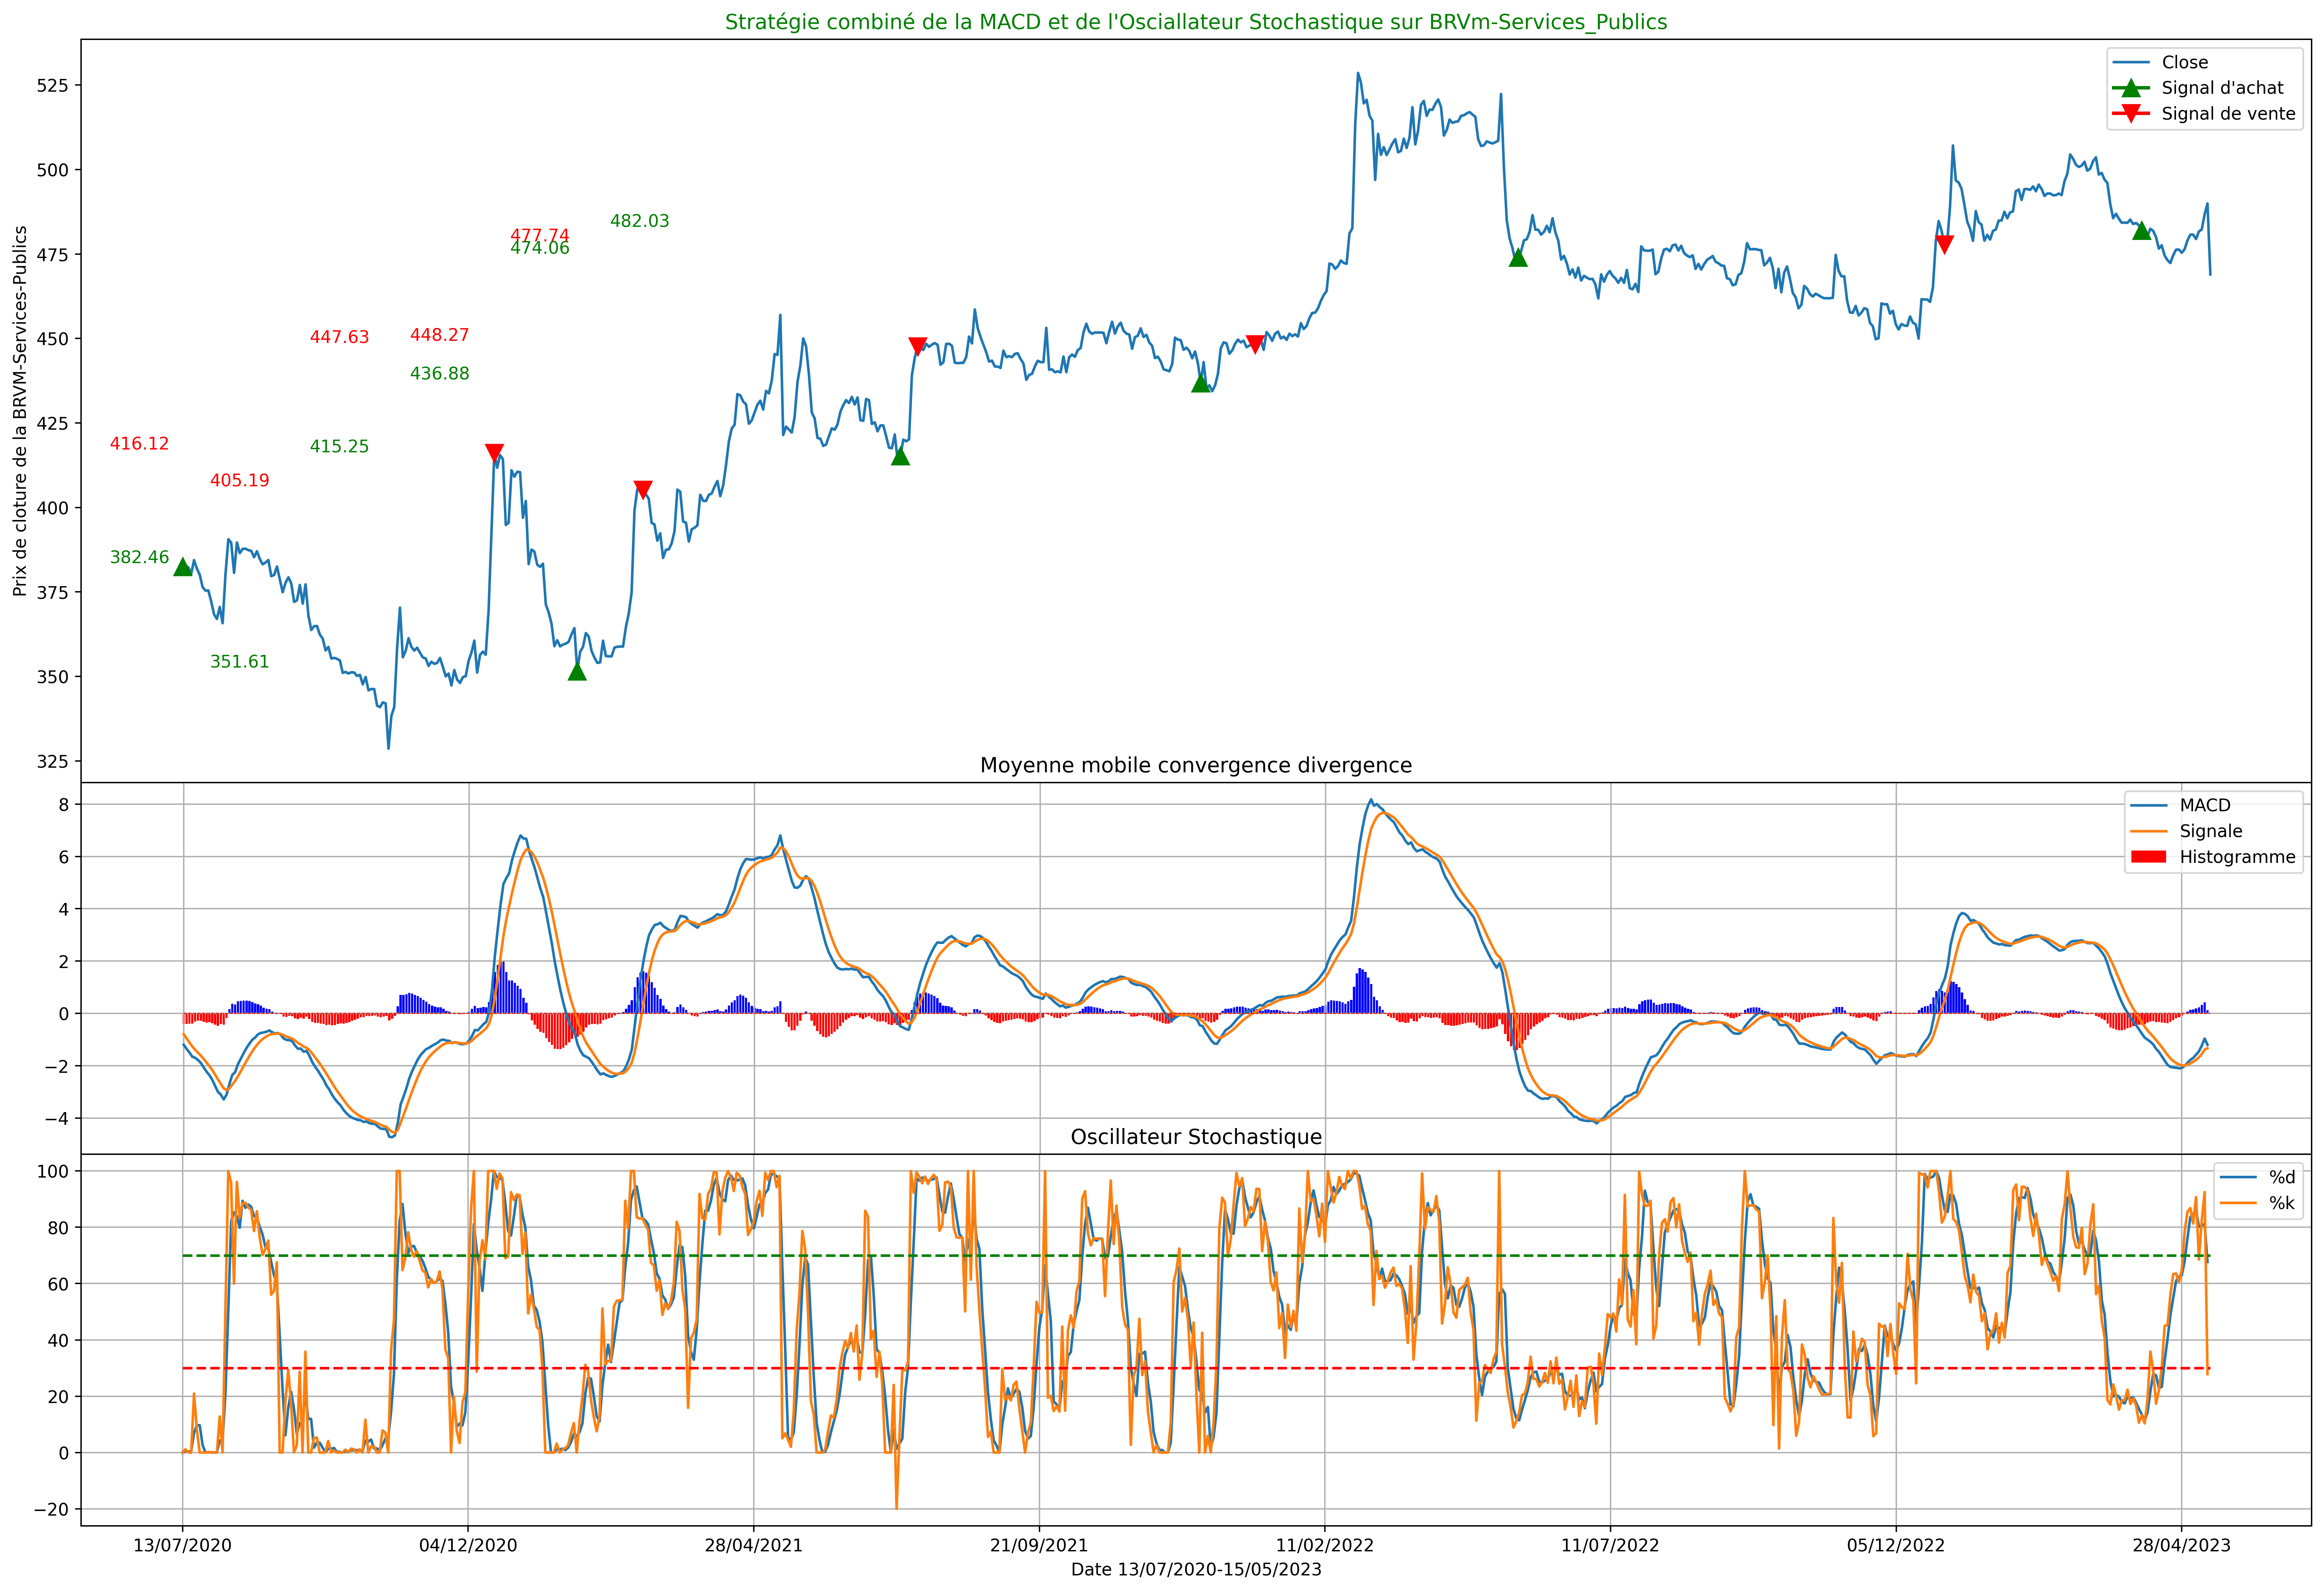
\includegraphics[width=1 \textwidth ]{img/MACD-Public.png}
    \caption{Strategie des Moyennes Mobiles sur la BRVM-Services-Publics}
    \label{fig:Strategie des Moyennes Mobiles sur la BRVM-Services-Publics}
\end{figure}

\par{La figure ci-dessus présente l'application de la stratégie combinée de l'oscillateur 
Stochastique et de la Moyenne Mobile Convergence Divergence sur l'indice BRVM-Service-Publics.
De son analyse il ressort qu'il y a une répartition équitable des signaux d'achat et de vente
générer par la Moyenne Mobile Convergence Divergence. En tout nous avons obtenu 
9 signaux d'achat et de vente dont un signal d'achat final. La transaction
la plus bénéfique réalisé est la deuxième ou le prix d'achat de la valeur était 
de 351,61 Fcfa et son prix de vente de 405,19 Fcfa. Notons que toutes les transactions 
sont positives et que le taux de bénéfice total réalisé à la fin de l'application de 
la stratégie est de \textbf{39,758\&}.

Bien que toute les transaction soit 
positive on observe que le 5eme signal de vente est venu un peut trop tôt 
car dans la suite de l'évolution des cours, le prix de l'indice à dépasser les 
500 Fcfa contre un signal d'achat ou l'indice coutait 474,06 Fcfa. Ce retard est 
d'autant plus remarquable au niveau de la 4eme transaction où le signal de vente est 
venu vraiment très tôt cas juste après le signal de vente l'indice à atteint sont 
cours maximal de \textbf{ 528,59 Fcfa}.}




\subsection{{Interprétation des résultats et vérifications des hypothèses.}}

D'après les analyses, la stratégie des Moyennes Mobile sur l'indice BRVM-Agriculture à 
générer au total de 8 signaux d'achat et de vente et 6 signaux d'achat et de vente 
sur l'indice BRVM-Services-Publics. En ce qui concerne la stratégie
combinée de l'Oscillateur Stochastique et de la Moyenne Mobile Convergence Divergence, 
elle à donner 13 signaux d'achat et de vente pour l'indice BRVM-Agriculture et 
11 signaux d'achat et de vente pour l'indice BRVM-Services-Publics, ce qui fait un total
de 24 signaux. Nous remarquons donc que nombre total de signaux obtenu grâce 
à la stratégie des Moyennes Mobiles ainsi que le nombre total de signaux individuel pour 
chaque indice est inférieur aux signaux obtenu grâce à la stratégie combiné de l'oscillateur
stochastique et de la Moyenne Mobile Convergence Divergence. Alors l'hypothèses selon laquelle 
la méthode des Moyennes Mobiles génère plus de signal d'achat et de ventes que la méthodes
combinée de l'Oscillateur Stochastique et de la des Moyennes Mobiles convergence divergence 
n'est pas vérifier.

De plus il ressort que l'application de la stratégie des moyennes 
mobile à générer un bénéfice total de 367,167\% sur l'indice BRVM-Agriculture et 
un total de 18,01\% sur l'indice BRVM-Services-Publics. Par ailleurs la stratégie 
combinée de l'Oscillateur Stochastique et de la Moyenne Mobile Convergence Divergence
quand à elle a donné un bénéfice total de 29,105\% sur l'indice BRVM-Agriculture 
contre un bénéfice total de 39,758\% pour l'indice BRVM-Service-Publics. 
Il ressort de ces résultats que \textbf{la stratégie des Moyennes Mobile donne plus de 
bénéfice sur l'indice BRVM-Agriculture que sur l'indice BRVM-Services-Publics. 
Alors que la stratégie Combiné de l'Oscillateur Stochastique et de la 
Moyenne Mobile Convergence Divergence donne plus de bénéfices sur 
l'indice BRVM-Service-Public que sur l'indice BRVM-Agriculture}. En somme 
la stratégie des Moyennes Mobiles donne un total de 385,177\% pour les deux indices 
et la méthode combinée de l'Oscillateur Stochastique et de la Moyenne Mobile Convergence Divergence
produit un total de 68,863\% pour les deux indices. Alors l'hypothèses selon laquelle
la  méthode combinée de l'Oscillateur Stochastique et de la Moyenne Mobile Convergence Divergence
génère plus de bénéfices que la méthode des Moyennes Mobile n'est pas vérifié.

\section{Approche de solution}
\par{
Afin d'optimiser au mieux le profil des investisseurs à la Bourse Régional des 
valeurs Mobilière, notamment ceux qui investissent dans le domaine des Services
Publics et de l'Agriculture, entre la stratégie de la 
moyenne mobile et de la méthode Combiné de l'Oscillateur Stochastique et de la 
Moyenne Mobile Convergence Divergence au vu des résultats obtenus dans cet études 
nous recommandons vivement l'utilisation de la stratégie des Moyennes Mobile 
sur l'indice BRVM-Agriculture et l'usage de la méthode Combiné de l'Oscillateur
    stochastique et de la Moyenne Mobile Convergence Divergence sur l'indice 
    BRVM-Services-Publics. De plus dans le cadre de l'application de ces stratégies
    nous recommandons de faire des simulations afin de déterminer les paramètres pour la stratégie des 
    moyennes mobiles qui permettent d'obtenir de meilleur bénéfice pour les tendance 
    futur du marché et l'usage de nos critère de validations des paramètres élaborer dans le 
    cadre de cette étude comparative. 
}





\end{itemize}
